\documentclass[sigconf,authordraft,nonacm]{acmart}

\AtBeginDocument{%
  \providecommand\BibTeX{{%
    Bib\TeX}}}

\usepackage{booktabs}
\usepackage{graphicx}
\usepackage{microtype}
\usepackage{tabularx}
\usepackage{array}

\setlength{\columnsep}{12pt}
\setlength{\emergencystretch}{2em}

\title[SnapCal Report]{SnapCal: SAM-Guided Food Recognition and Calorie Estimation from Meal Photographs}

\author{Jay Malve}
\email{jama1639@colorado.edu}
\affiliation{%
  \institution{University of Colorado Boulder}
  \city{Boulder}
  \state{Colorado}
  \country{USA}
}

\renewcommand{\shortauthors}{Malve}

\begin{abstract}
SnapCal is an end-to-end food recognition and calorie estimation system built around Food-101 image classification, USDA nutrition lookup, and a web-based inference workflow. The original project goal was to test whether Segment Anything Model (SAM) guided food isolation could improve classification accuracy and downstream calorie estimation reliability compared to raw-image baselines. To support that goal, the project implemented a reproducible research pipeline that generated Food-101 manifests, supported MobileSAM preprocessing, trained ResNet-50, EfficientNet-B0, and ViT-B/16 classifiers, exported inference bundles, served predictions through a Django API, and exposed the workflow through a Next.js frontend with portion-size control. The strongest fully verified experiment in the repository is a local ResNet-50 raw-image baseline trained on the full Food-101 test split, which achieved 84.83\% top-1 accuracy, 97.00\% top-5 accuracy, and 0.848 macro F1 on 25,250 test images. To probe the segmentation question within local compute limits, this report also includes a matched ResNet-50 pilot ablation on a reduced 808-image stratified manifest. In that pilot, segmented inputs underperformed raw inputs, dropping top-1 accuracy from 15.84\% to 11.88\% and macro F1 from 0.112 to 0.096. The report therefore documents a completed end-to-end system, a strong verified full-dataset baseline, and a preliminary local segmentation result, while deferring full cross-architecture and calorie-estimation studies to future work.
\end{abstract}

\keywords{food recognition, calorie estimation, computer vision, MobileSAM, Vision Transformer, Django, Next.js}

\begin{document}

\maketitle

\section{Introduction}
Estimating the nutritional content of a meal from a photograph is a useful computer vision problem with practical applications in dietary tracking, health monitoring, and consumer-facing nutrition tools. In real-world meal photos, however, food often appears with cluttered backgrounds such as plates, napkins, utensils, tabletops, and hands. Those extra visual elements can make classification harder and can reduce confidence in downstream nutrition estimates.

This project studied whether food-first preprocessing could improve recognition quality. The original proposal centered on a distilled Segment Anything Model (SAM) pipeline that would isolate food regions before classification, followed by a model that mapped the predicted class to USDA nutrition values for calorie and macronutrient estimation. The project also aimed to compare segmented and unsegmented inputs across transformer and convolutional architectures.

The final implemented system grew into a complete monorepo that covered offline preprocessing, model training, evaluation, export, backend serving, and frontend interaction. The backend was fully implemented in Django, and the user workflow included portion-size adjustment so that standard-serving nutrition values could be scaled at inference time. However, full segmented preprocessing over all 101,000 Food-101 images was not practical on the available local hardware, so this report presents two levels of evidence instead of a complete experiment matrix: a verified full-dataset raw baseline and a smaller local ResNet-50 pilot ablation on a reduced stratified manifest. This report therefore documents both the completed engineering work and the current, compute-constrained experimental evidence.

\section{Related Work and Background}
Food recognition has been studied as a fine-grained visual classification problem because many meal categories share similar colors, textures, and presentation styles. Food-101 is a standard benchmark for this setting because it contains 101 classes with substantial intra-class variation and strong background diversity \cite{bossard2014food101}.

Modern transfer learning methods provide strong starting points for this task. ResNet-50 remains a common convolutional baseline because residual connections enable deep image classifiers to train effectively \cite{he2016resnet}. EfficientNet-B0 provides a lighter-weight CNN family that emphasizes efficiency through compound scaling \cite{tan2019efficientnet}. Vision Transformers have also become competitive image classifiers by modeling images as patch sequences and leveraging large-scale pretraining \cite{dosovitskiy2021vit}.

Segmentation is a natural preprocessing step for meal images because it can suppress irrelevant context before classification. Segment Anything introduced a foundation-model approach to generic segmentation \cite{kirillov2023sam}, and MobileSAM made that idea more practical for resource-constrained workflows \cite{mobilesam2023}. In SnapCal, the segmentation stage was not treated as the final task itself; instead, it acted as a front-end filter designed to isolate food pixels, improve focus on the meal, and potentially boost classifier robustness.

The nutrition stage relied on USDA FoodData Central \cite{usdafdc}, which provided serving-based calorie and macronutrient references. Rather than attempting direct calorie regression from pixels, the project used a class-to-nutrition mapping approach: first classify the meal, then retrieve nutrition estimates for a standard serving, then scale the result by portion multiplier. This design made the system easier to inspect, debug, and extend.

\section{Methodology}

\subsection{Dataset}
The project used Food-101 \cite{bossard2014food101}, which contains 101,000 images across 101 food categories. The repository generated a canonical manifest file from the Food-101 metadata and then split the official training data into training and validation subsets with a deterministic class-wise shuffle. The resulting manifest contained 68,175 training images, 7,575 validation images, and 25,250 test images. Each manifest row stored the class label, image path, and reserved output paths for segmentation products.

Table~\ref{tab:dataset-summary} summarizes the dataset organization used by the pipeline.

\begin{table}
  \caption{Dataset summary used by SnapCal. Counts are taken from the generated manifest tracked in the repository.}
  \label{tab:dataset-summary}
  \begin{tabular}{lrr}
    \toprule
    Split & Image count & Notes \\
    \midrule
    Train & 68,175 & Deterministic split from official Food-101 training set \\
    Validation & 7,575 & Held out from official training set \\
    Test & 25,250 & Official Food-101 test set \\
    \midrule
    Total & 101,000 & 101 classes \\
    \bottomrule
  \end{tabular}
\end{table}

In addition to the full manifest, the project generated a reduced local pilot manifest for the preliminary SAM ablation reported later in this paper. That pilot kept all 101 classes but sampled only 5 training images, 1 validation image, and 2 test images per class, for 808 total images. The pilot manifest was used only for the matched raw-versus-segmented ResNet-50 comparison and is reported separately from the full-dataset baseline so that the two result types are not conflated.

\subsection{SAM-Guided Segmentation Pipeline}
The segmentation stage was implemented with MobileSAM. For each input image, the pipeline generated candidate masks, filtered them by minimum area and area ratio, ranked them using a weighted score, and selected the most prominent one or two masks for composition. The ranking score combined mask area ratio, predicted IoU, stability score, and a center-distance penalty so that large, confident, centrally located food regions were preferred.

After mask selection, the system combined the chosen masks, replaced the background with an ImageNet-style fill color, cropped around the selected region with a small margin, and resized the result to 224\,$\times$\,224 pixels. The segmentation code also exported mask metadata such as candidate counts, bounding boxes, mask scores, and retained area ratios so that the preprocessing stage remained inspectable.

The manifest paths and segmentation tooling were fully implemented, and the pipeline was exercised end-to-end on a reduced local pilot manifest. However, a full segmented preprocessing pass over the entire 101,000-image dataset remained impractical on the available local hardware. As a result, this report includes a preliminary segmented-input pilot ablation rather than a full segmented-dataset sweep.

\subsection{Classification Models}
SnapCal supported three pretrained classifier families:

\begin{itemize}
\item ResNet-50 as the main CNN baseline \cite{he2016resnet}
\item EfficientNet-B0 as a lighter-weight efficiency baseline \cite{tan2019efficientnet}
\item ViT-B/16 as the transformer-based model \cite{dosovitskiy2021vit}
\end{itemize}

The training pipeline was config-driven and loaded one of the three model families based on a JSON experiment file. For ResNet-50 and EfficientNet-B0, the classification head was replaced with a 101-class layer. For ViT-B/16, the Hugging Face Transformers implementation loaded a pretrained ViT-B/16 checkpoint and replaced the classifier head to match Food-101 labels \cite{transformers}.

\subsection{Training Procedure}
The shared base training configuration used image size 224, batch size 64, 15 epochs, AdamW with learning rate $3 \times 10^{-4}$, weight decay 0.01, and label smoothing 0.1. The learning rate scheduler used cosine annealing. The training augmentations included random horizontal flip, random rotation up to 15 degrees, color jitter, and random erasing. A reduced local configuration was used for the verified full-dataset baseline reported in this paper; that run used batch size 16, 3 epochs, and zero data-loader workers to fit a self-contained local workflow. The same reduced training settings were also reused for the preliminary pilot ablation, but on the 808-image sampled manifest described above.

Table~\ref{tab:training-config} summarizes the three configuration levels most relevant to this report.

\begin{table}
  \caption{Training configuration summary for the base setup, the verified local baseline, and the matched pilot ablation.}
  \label{tab:training-config}
  \footnotesize
  \setlength{\tabcolsep}{3pt}
  \begin{tabularx}{\columnwidth}{@{}>{\raggedright\arraybackslash}p{0.23\columnwidth}>{\centering\arraybackslash}p{0.16\columnwidth}>{\centering\arraybackslash}p{0.24\columnwidth}>{\centering\arraybackslash}p{0.23\columnwidth}@{}}
    \toprule
    Setting & Base & Verified & Pilot \\
    \midrule
    Model & Config-dependent & ResNet-50 & ResNet-50 \\
    Input variant & Raw or segmented & Raw & Raw and segmented \\
    Manifest & Full Food-101 & Full Food-101 & 808-image subset \\
    Image size & 224 & 224 & 224 \\
    Batch size & 64 & 16 & 16 \\
    Epochs & 15 & 3 & 3 \\
    Learning rate & 0.0003 & 0.0003 & 0.0003 \\
    Optimizer & AdamW & AdamW & AdamW \\
    Scheduler & Cosine annealing & Cosine annealing & Cosine annealing \\
    Label smoothing & 0.1 & 0.1 & 0.1 \\
    \bottomrule
  \end{tabularx}
\end{table}

For the pilot ablation, the segmentation stage used a faster local MobileSAM configuration with fewer prompt points and no crop-layer recursion so that preprocessing could finish within a single local work session. That speed-oriented setting is useful for a preliminary ablation, but it is not equivalent to a final full-dataset segmentation study.

\subsection{Nutrition and Calorie Estimation}
The calorie estimation stage mapped each Food-101 class to an entry in USDA FoodData Central \cite{usdafdc}. Each mapping row stored serving size, calories, protein, carbohydrates, fat, and metadata about mapping confidence. At inference time, the system returned the top predictions, looked up the corresponding standard-serving nutrition facts, and then scaled those values by a user-selected portion multiplier.

This design kept the calorie pipeline interpretable because it made every nutrition estimate traceable to a specific class prediction and a specific reference entry. At the same time, it introduced a dependency on the quality of the Food-101-to-USDA mapping table. In the repository version used for this report, 74 of 101 classes were populated with auto-filled USDA matches, while 27 classes were still marked for manual curation. That incomplete coverage, together with the missing external calorie-evaluation protocol, is the main reason calorie MAE remains future work in this report.

\subsection{System Architecture and Implementation}
The final system was implemented as a monorepo with four main layers:

\begin{itemize}
\item offline research scripts for manifest generation, segmentation, training, evaluation, and bundle export
\item a shared Python package that contained datasets, model builders, evaluation utilities, segmentation helpers, and nutrition logic
\item a Django REST backend that served health and prediction endpoints
\item a Next.js frontend that handled image upload, camera capture, result display, and portion-size adjustment
\end{itemize}

The backend loaded an exported inference bundle containing the model weights, metadata, optional segmentation config, and nutrition mapping. The frontend sent an image and portion multiplier to the API, and the API returned the selected class, top predictions, nutrition facts, and latency metrics. This architecture aligned with the original goal of deploying an end-to-end meal analysis application, even though the strongest fully verified full-dataset experiment in this report focused on the raw-image baseline.

Figure~\ref{fig:pipeline} shows the system pipeline at a high level.

\begin{figure}
  \centering
  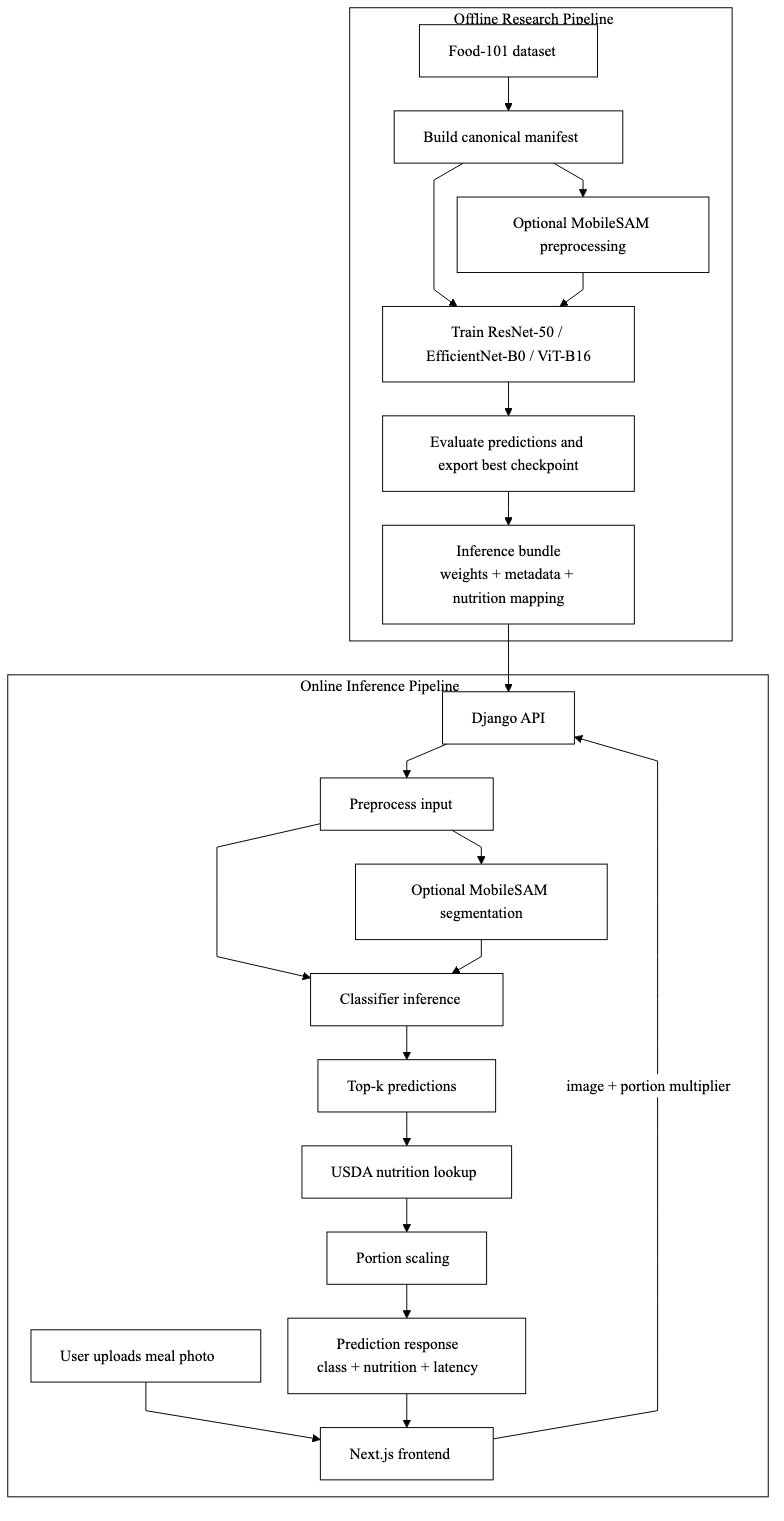
\includegraphics[width=0.95\linewidth]{figures/pipeline.png}
  \caption{High-level SnapCal pipeline showing the offline research workflow and the online inference path.}
  \Description{Diagram showing the SnapCal offline research pipeline from Food-101 dataset to manifest generation, optional MobileSAM preprocessing, model training, evaluation, and exported inference bundle, followed by the online inference pipeline from user upload through the Next.js frontend, Django API, optional segmentation, classifier inference, USDA nutrition lookup, portion scaling, and prediction response.}
  \label{fig:pipeline}
\end{figure}

\section{Experiments and Results}

\subsection{Evaluation Metrics}
The evaluation pipeline computed top-1 accuracy, top-5 accuracy, macro F1, per-class precision, recall, and F1, as well as a full confusion matrix. These metrics were generated directly from saved top-$k$ predictions. For runtime evaluation, the inference service also reported preprocessing, inference, and total latency in milliseconds.

\subsection{Verified Baseline Result}
The strongest verified experiment present in the repository at the time of writing was the local raw-image ResNet-50 baseline report for the full-dataset raw run. That experiment achieved 84.8277\% top-1 accuracy, 97.0020\% top-5 accuracy, and 0.848108 macro F1 on the 25,250-image Food-101 test split.

Table~\ref{tab:baseline-results} summarizes the verified baseline.

\begin{table}
  \caption{Current verified baseline result from the repository.}
  \label{tab:baseline-results}
  \begin{tabular}{lcccc}
    \toprule
    Model & Input & Epochs & Top-1 & Top-5 \\
    \midrule
    ResNet-50 & Raw & 3 & 84.83\% & 97.00\% \\
    \bottomrule
  \end{tabular}
\end{table}

This baseline was important for two reasons. First, it established that the training, evaluation, and export pipeline produced a competitive Food-101 model even before any segmented-input comparison was completed. Second, it provided a strong reference point for the overall quality of the raw-image classification pipeline. The top-1 result also landed close to the original project goal of 85\% accuracy, which suggested that the core classification pipeline was viable. Because the pilot ablation reported next uses a much smaller manifest, its results are analyzed separately rather than being compared directly to this full-dataset baseline.

\subsection{Per-Class Behavior}
Per-class F1 analysis showed that some categories were classified very reliably, while others remained difficult because of visual similarity across dishes. The five strongest classes in the verified baseline were edamame (0.992), macarons (0.970), oysters (0.952), hot and sour soup (0.950), and miso soup (0.945). The five weakest classes were pork chop (0.580), steak (0.618), chocolate mousse (0.660), apple pie (0.668), and bread pudding (0.687).

Table~\ref{tab:perclass-extremes} summarizes these extremes.

\begin{table}
  \caption{Best and worst per-class F1 scores for the verified ResNet-50 raw baseline.}
  \label{tab:perclass-extremes}
  \begin{tabular}{lr}
    \toprule
    Class & F1 \\
    \midrule
    Edamame & 0.992 \\
    Macarons & 0.970 \\
    Oysters & 0.952 \\
    Hot and sour soup & 0.950 \\
    Miso soup & 0.945 \\
    \midrule
    Pork chop & 0.580 \\
    Steak & 0.618 \\
    Chocolate mousse & 0.660 \\
    Apple pie & 0.668 \\
    Bread pudding & 0.687 \\
    \bottomrule
  \end{tabular}
\end{table}

The lowest-performing classes matched common fine-grained failure modes. Several dishes shared similar plating styles, brown or cream color palettes, and overlapping textures. This pattern supports the original motivation for trying segmentation: when background clutter and plate context are reduced, borderline categories may become easier to separate.

\subsection{Confusion Patterns}
The confusion matrix highlighted several visually intuitive failure pairs. The largest confusions in the verified baseline included pork chop mistaken for steak (34), filet mignon mistaken for steak (34), tuna tartare mistaken for beef tartare (33), chocolate cake mistaken for chocolate mousse (31), and steak mistaken for filet mignon (30). These errors were consistent with categories that share preparation style, texture, or dominant color.

\begin{table}
  \caption{Largest confusion pairs in the verified ResNet-50 raw baseline.}
  \label{tab:confusions}
  \begin{tabular}{lr}
    \toprule
    True class $\rightarrow$ predicted class & Count \\
    \midrule
    Pork chop $\rightarrow$ steak & 34 \\
    Filet mignon $\rightarrow$ steak & 34 \\
    Tuna tartare $\rightarrow$ beef tartare & 33 \\
    Chocolate cake $\rightarrow$ chocolate mousse & 31 \\
    Steak $\rightarrow$ filet mignon & 30 \\
    \bottomrule
  \end{tabular}
\end{table}

These confusion patterns provide a concrete target for both the preliminary segmented-input pilot and any future full-dataset segmented evaluation. If segmentation removes distracting dishware and background cues while preserving food texture and shape, the hardest classes should show the clearest gains.

\subsection{Preliminary SAM Segmentation Ablation}
To evaluate the segmented-input path within local compute limits, the project ran a matched ResNet-50 pilot ablation on the reduced 808-image stratified manifest described earlier. Both pilot runs used the same 3-epoch local training settings and the same sampled raw images; the only difference was whether the input images were fed directly to the classifier or first processed with the faster local MobileSAM configuration.

\begin{table*}
  \caption{Preliminary local ResNet-50 SAM ablation on the reduced 808-image pilot manifest.}
  \label{tab:sam-ablation}
  \begin{tabular}{lcccccc}
    \toprule
    Model & Raw top-1 & Segmented top-1 & Raw top-5 & Segmented top-5 & Raw macro F1 & Segmented macro F1 \\
    \midrule
    ResNet-50 pilot & 15.84\% & 11.88\% & 38.61\% & 29.21\% & 0.112 & 0.096 \\
    \bottomrule
  \end{tabular}
\end{table*}

Under this constrained pilot, segmentation did not improve the aggregate metrics. Compared with the raw-input pilot run, segmented inputs reduced top-1 accuracy by 3.96 percentage points, reduced top-5 accuracy by 9.41 percentage points, and reduced macro F1 by 0.016. This is still a preliminary result rather than a definitive answer to the original research question. The pilot test split contains only 2 images per class, which makes class-level statistics too unstable for strong per-class claims, and the segmentation config was deliberately simplified to keep runtime manageable on local hardware. The main value of this pilot is therefore twofold: it verifies that the full segmented preprocessing, training, and evaluation path works end-to-end, and it provides an honest early signal that segmentation did not help under this small local setting.

\subsection{Cross-Architecture Comparison}
The repository already supported ResNet-50, EfficientNet-B0, and ViT-B/16 training through config-driven experiments, but a fair cross-architecture matrix would require either full-dataset segmented preprocessing or matched reduced-manifest pilot runs for all three backbones. Given the available local compute budget, this report intentionally defers that comparison to future work instead of mixing full-dataset ResNet-50 results with pilot-scale segmented results. The next logical extension would be to repeat the same reduced-manifest pilot protocol for EfficientNet-B0 and ViT-B/16, then move the final six-run raw-versus-segmented matrix to GPU-backed hardware.

\subsection{Calorie Estimation Accuracy}
Calorie mean absolute error remains future work. In addition to the incomplete Food-101-to-USDA mapping table, the project still needs a clearly defined calorie-evaluation protocol so that the same lookup table is not reused as both the prediction source and the evaluation target. In the repository version used for this report, 74 classes had populated USDA matches and 27 still required manual curation, so reporting calorie MAE as a finished metric would overstate confidence.

\begin{table}
  \caption{Current status of the calorie estimation evaluation path.}
  \label{tab:calorie-results}
  \footnotesize
  \setlength{\tabcolsep}{3pt}
  \begin{tabularx}{\columnwidth}{@{}>{\raggedright\arraybackslash}p{0.34\columnwidth}X@{}}
    \toprule
    Metric & Value \\
    \midrule
    Classes with populated USDA mapping & 74 / 101 \\
    Calorie MAE status & Deferred until mapping curation and evaluation protocol are finalized \\
    Portion-scaling evaluation note & Implemented in the product workflow; not yet benchmarked against external calorie labels \\
    \bottomrule
  \end{tabularx}
\end{table}

\subsection{Latency and Deployment Notes}
The deployed inference architecture was fully implemented around a Django backend and a Next.js frontend. The backend loaded an exported model bundle and returned latency measurements for preprocessing and inference. In local warm-start testing with the exported production bundle, repeated single-image inference calls fell well below the original two-second response target, while the first call remained slower because it included model loading overhead. This distinction matters for deployment because user-perceived latency after service warm-up is more representative than cold-start timing.

Figure~\ref{fig:frontend} is reserved for a final application screenshot.

\begin{figure}
  \centering
  \fbox{\parbox[c][1.4in][c]{0.95\linewidth}{\centering
  Placeholder screenshot for the final frontend.\\
  Replace with the SnapCal UI showing image upload, predicted class, nutrition results, and portion-size control.}}
  \caption{Frontend placeholder. A future revision can replace this box with a screenshot of the completed SnapCal interface.}
  \Description{A placeholder screenshot box for the SnapCal frontend showing upload controls, prediction output, nutrition values, and portion-size adjustment.}
  \label{fig:frontend}
\end{figure}

\section{Discussion}
Several aspects of the project worked well. First, the repository matured into a complete end-to-end system rather than stopping at an isolated notebook experiment. The project implemented manifest generation, optional segmentation, model training, evaluation, bundle export, API inference, and frontend interaction in a single reproducible codebase. Second, the verified ResNet-50 raw baseline was strong enough to validate the core learning setup. A top-1 accuracy of 84.83\% and top-5 accuracy of 97.00\% indicated that the training and evaluation pipeline was functioning well and that transfer learning on Food-101 was effective.

The project also surfaced several limitations. The most important experimental limitation was compute scale. The report now includes a preliminary segmented-input pilot ablation, but that study was run on a reduced 808-image manifest with a speed-oriented local segmentation config rather than on the full Food-101 dataset. That means the central research question --- whether SAM-guided preprocessing materially improves recognition quality at full scale --- is still only partially answered in this version. Similarly, the calorie-estimation stage depended on a mapping table that still required manual curation for part of the label set and on an evaluation protocol that had not yet been formalized, which prevented a strong calorie MAE claim.

Another useful insight is that the project evolved slightly from the original proposal while still preserving its core goal. The proposal described a FastAPI backend, but the final production backend was implemented in Django. That change did not weaken the system; in practice, the Django API cleanly exposed health and prediction endpoints and integrated well with the exported bundle format. The project also finalized portion-size support as part of the application workflow so that nutrition output could be scaled beyond the default serving size.

Overall, the baseline results and system implementation suggest that the project succeeded as both a research platform and a deployable prototype. The report now contains both a strong verified full-dataset raw baseline and a preliminary local raw-versus-segmented pilot, but the final full-scale segmentation question remains future work rather than a closed result.

\section{Conclusion and Future Work}
This project presented SnapCal, a food recognition and calorie estimation system built around Food-101 classification, optional MobileSAM preprocessing, USDA nutrition lookup, a Django inference backend, and a Next.js frontend. The completed implementation covered the full path from raw image input to portion-adjusted nutrition output. The strongest currently verified model in the repository, a raw-image ResNet-50 baseline, achieved 84.83\% top-1 accuracy and 97.00\% top-5 accuracy on the Food-101 test set, demonstrating that the classification backbone of the system was already strong.

To probe the segmentation question under realistic local compute constraints, the project also ran a matched ResNet-50 pilot ablation on a reduced 808-image manifest. In that pilot, segmented inputs underperformed raw inputs, achieving 11.88\% top-1 accuracy versus 15.84\% for the raw-input pilot. Because the pilot used only two test examples per class and a speed-oriented local segmentation config, it should be interpreted as a preliminary signal rather than a definitive answer. Future work should rerun the segmentation study on the full Food-101 dataset with GPU-backed preprocessing, extend the same protocol to EfficientNet-B0 and ViT-B/16, and define a stricter calorie-evaluation protocol after the USDA mappings are fully curated.

\begin{acks}
This report used the course-provided ACM template structure as a starting point and was adapted into a class project report format. The SnapCal codebase integrates research components, deployment utilities, and application code across Python, Django, and Next.js.
\end{acks}

\bibliographystyle{ACM-Reference-Format}
\bibliography{references}

\appendix

\section{Implementation Snapshot}
The repository snapshot used for this report contained the following report-relevant evidence:

\begin{itemize}
\item a canonical Food-101 manifest with 101,000 total rows
\item completed segmentation code and configuration for MobileSAM preprocessing
\item config-driven model support for ResNet-50, EfficientNet-B0, and ViT-B/16
\item a verified local experiment report for the full-dataset raw ResNet-50 baseline
\item paired pilot reports for the reduced-manifest raw and segmented ResNet-50 ablation
\item an exported production bundle for backend inference
\item a Django API and Next.js frontend wired for image-based inference
\end{itemize}

\section{Open Follow-Ups}
The main remaining follow-up items after this report are:

\begin{itemize}
\item rerun the SAM raw-versus-segmented ablation on the full Food-101 dataset with GPU-backed preprocessing
\item extend the matched pilot protocol to EfficientNet-B0 and ViT-B/16 before building a final cross-architecture matrix
\item finalize the calorie MAE protocol and curate the remaining USDA mappings
\item a polished pipeline diagram
\item a real frontend screenshot including portion-size control
\end{itemize}

\end{document}
